\documentclass[tikz,border=8pt]{standalone}
\usepackage[T1]{fontenc}
\usepackage{helvet}
\renewcommand{\familydefault}{\sfdefault}
\usetikzlibrary{arrows.meta,positioning,fit,calc,backgrounds}

\definecolor{ink}{HTML}{1F2933}
\definecolor{fast}{HTML}{D9480F}
\definecolor{fastbg}{HTML}{FFF4E6}
\definecolor{slow}{HTML}{1864AB}
\definecolor{slowbg}{HTML}{E7F5FF}
\definecolor{mem}{HTML}{2B8A3E}
\definecolor{membg}{HTML}{EBFBEE}
\definecolor{host}{HTML}{5F3DC4}
\definecolor{hostbg}{HTML}{F3F0FF}
\definecolor{off}{HTML}{868E96}
\definecolor{offbg}{HTML}{F1F3F5}

\begin{document}
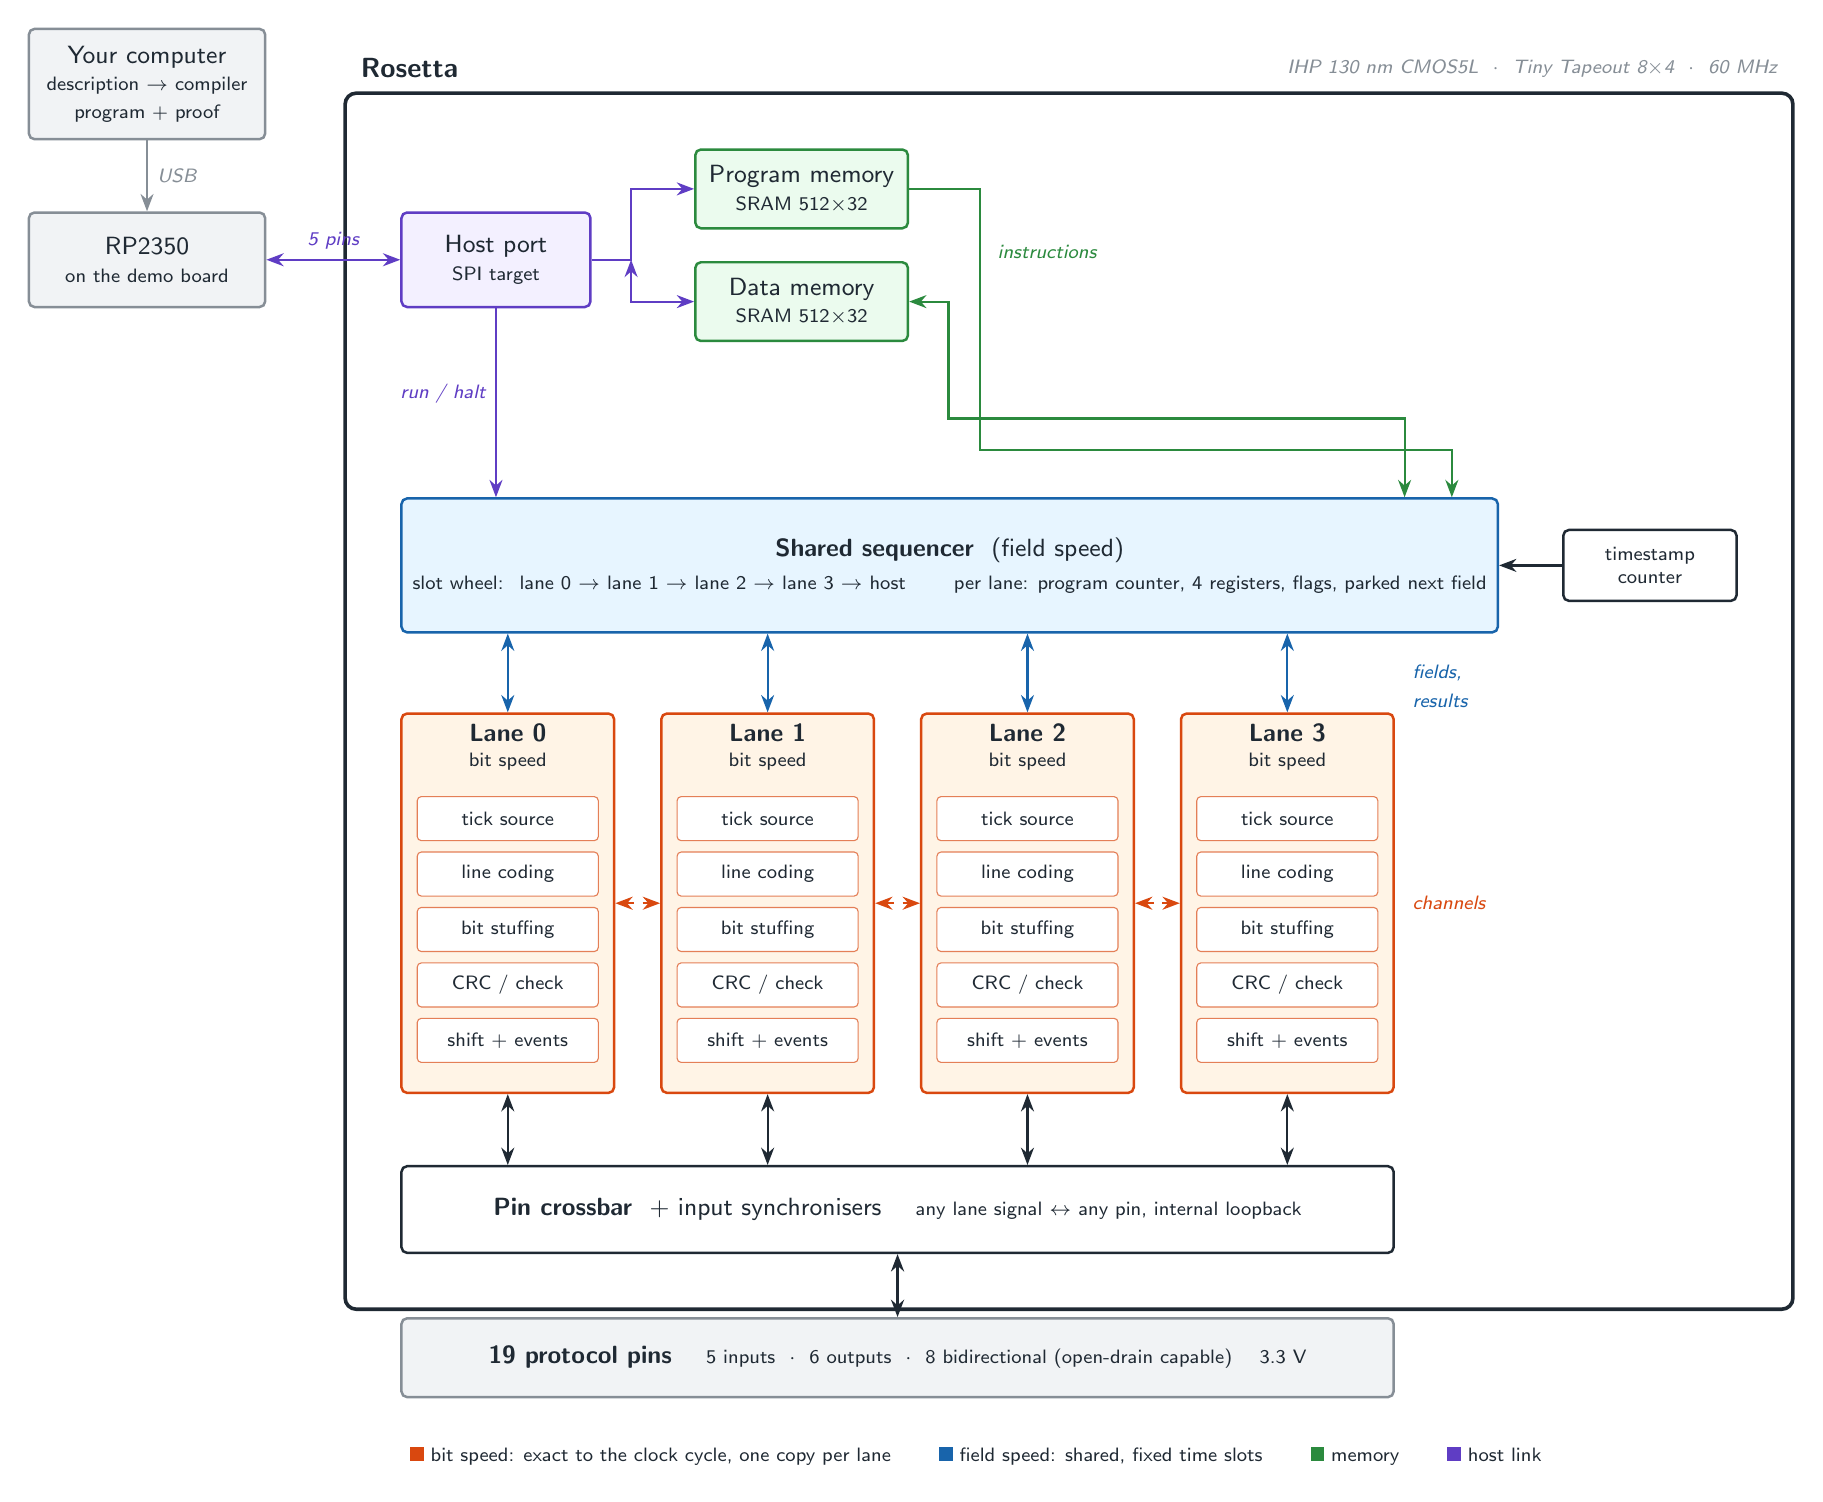
\begin{tikzpicture}[
  font=\small, text=ink, >={Stealth[length=2.2mm]},
  box/.style={draw=#1, line width=0.9pt, rounded corners=2pt, align=center,
              minimum height=10mm, inner sep=4pt},
  lane/.style={box=fast, fill=fastbg, minimum width=27mm, minimum height=47mm,
               align=center, text depth=40mm},
  item/.style={draw=fast!70, fill=white, rounded corners=1.5pt, font=\scriptsize,
               minimum width=23mm, minimum height=5.6mm, inner sep=1pt},
  wire/.style={line width=0.8pt, draw=ink},
  note/.style={font=\scriptsize\itshape, text=off},
]

% ---------------- off-chip (left) ----------------
\node[box=off, fill=offbg, minimum width=30mm, minimum height=14mm] (pc)
  {Your computer\\[-1pt]\scriptsize description $\rightarrow$ compiler\\[-1pt]\scriptsize program + proof};
\node[box=off, fill=offbg, minimum width=30mm, minimum height=12mm, below=9mm of pc] (rp)
  {RP2350\\[-1pt]\scriptsize on the demo board};
\draw[wire, off, ->] (pc) -- node[right, note]{USB} (rp);

% ---------------- host port ----------------
\node[box=host, fill=hostbg, minimum width=24mm, minimum height=12mm, right=17mm of rp] (hp)
  {Host port\\[-1pt]\scriptsize SPI target};
\draw[wire, host, <->] (rp) -- node[above, note, text=host]{5 pins} (hp);

% ---------------- memories ----------------
\node[box=mem, fill=membg, minimum width=27mm, right=13mm of hp, yshift=9mm] (pm)
  {Program memory\\[-1pt]\scriptsize SRAM 512$\times$32};
\node[box=mem, fill=membg, minimum width=27mm, below=4mm of pm] (dm)
  {Data memory\\[-1pt]\scriptsize SRAM 512$\times$32};
\draw[wire, host, ->] (hp.east) -- ++(5mm,0) |- (pm.west);
\draw[wire, host, <->] (hp.east) ++(5mm,0) |- (dm.west);

% ---------------- shared sequencer ----------------
\node[box=slow, fill=slowbg, minimum width=126mm, minimum height=17mm,
      below=24mm of hp.south west, anchor=north west] (seq)
  {\textbf{Shared sequencer} \ (field speed)\\[1pt]
   \scriptsize slot wheel: \ lane 0 $\rightarrow$ lane 1 $\rightarrow$ lane 2 $\rightarrow$ lane 3 $\rightarrow$ host
   \qquad per lane: program counter, 4 registers, flags, parked next field};
\draw[wire, mem, ->] (pm.east) -- ++(9mm,0) coordinate (pmr) |- ($(seq.north east)+(-6mm,6mm)$) -- ($(seq.north east)+(-6mm,0)$);
\draw[wire, mem, <->] (dm.east) -- ++(5mm,0) |- ($(seq.north east)+(-12mm,10mm)$) -- ($(seq.north east)+(-12mm,0)$);
\node[note, text=mem, anchor=west] at ($(pmr)+(1mm,-8mm)$) {instructions};
\draw[wire, host, ->] (hp.south) -- node[left, note, text=host, pos=0.45]{run / halt} (hp.south |- seq.north);

% ---------------- lanes ----------------
\foreach \i/\x in {0/0,1/33,2/66,3/99}{
  \node[lane, anchor=north west] (L\i) at ($(seq.south west)+(\x mm,-10mm)$) {\textbf{Lane \i}\\[-2pt]\scriptsize bit speed};
  \node[item] (a\i) at ($(L\i.north)+(0,-13.5mm)$) {tick source};
  \node[item, below=1.3mm of a\i] (b\i) {line coding};
  \node[item, below=1.3mm of b\i] (c\i) {bit stuffing};
  \node[item, below=1.3mm of c\i] (d\i) {CRC / check};
  \node[item, below=1.3mm of d\i] (e\i) {shift + events};
  \draw[wire, slow, <->] (L\i.north) -- (L\i.north |- seq.south);
}
\node[note, text=slow, anchor=west] at ($(L3.north east)+(1mm,5mm)$) {fields,};
\node[note, text=slow, anchor=west] at ($(L3.north east)+(1mm,1.5mm)$) {results};

% lane-to-lane channels
\draw[wire, fast, <->, dashed] (L0.east) -- (L1.west);
\draw[wire, fast, <->, dashed] (L1.east) -- (L2.west);
\draw[wire, fast, <->, dashed] (L2.east) -- (L3.west);
\node[note, text=fast, anchor=west] at ($(L3.east)+(1mm,0)$) {channels};

% ---------------- crossbar ----------------
\node[box=ink, fill=white, minimum width=126mm, minimum height=11mm,
      below=9mm of L0.south west, anchor=north west] (xb)
  {\textbf{Pin crossbar} \ + input synchronisers \quad \scriptsize any lane signal $\leftrightarrow$ any pin, internal loopback};
\foreach \i in {0,1,2,3}{ \draw[wire, <->] (L\i.south) -- (L\i.south |- xb.north); }

% timestamp
\node[box=ink, fill=white, minimum width=22mm, minimum height=9mm, font=\scriptsize,
      anchor=west] (ts) at ($(seq.east)+(8mm,0)$) {timestamp\\counter};
\draw[wire, ->] (ts.west) -- (seq.east);

% ---------------- pins ----------------
\node[box=off, fill=offbg, minimum width=126mm, minimum height=10mm,
      below=8mm of xb] (pins)
  {\textbf{19 protocol pins} \quad \scriptsize 5 inputs \ $\cdot$ \ 6 outputs \ $\cdot$ \ 8 bidirectional (open-drain capable) \quad 3.3 V};
\draw[wire, <->, line width=1.4pt] (xb) -- (pins);

% ---------------- chip outline ----------------
\begin{scope}[on background layer]
  \node[draw=ink, line width=1.3pt, rounded corners=4pt, fill=white,
        fit=(hp)(pm)(dm)(seq)(L0)(L3)(xb)(ts), inner sep=7mm] (chip) {};
\end{scope}
\node[anchor=south west, font=\bfseries] at ($(chip.north west)+(1mm,0.5mm)$) {Rosetta};
\node[anchor=south east, note] at ($(chip.north east)+(-1mm,0.5mm)$)
  {IHP 130 nm CMOS5L \ $\cdot$ \ Tiny Tapeout 8$\times$4 \ $\cdot$ \ 60 MHz};

% ---------------- legend ----------------
\node[anchor=north west, font=\scriptsize, align=left] at ($(pins.south west)+(0,-5mm)$)
  {\textcolor{fast}{\rule{1.6ex}{1.6ex}} bit speed: exact to the clock cycle, one copy per lane \qquad
   \textcolor{slow}{\rule{1.6ex}{1.6ex}} field speed: shared, fixed time slots \qquad
   \textcolor{mem}{\rule{1.6ex}{1.6ex}} memory \qquad
   \textcolor{host}{\rule{1.6ex}{1.6ex}} host link};
\end{tikzpicture}
\end{document}
